\documentclass[10pt, a4paper]{article}

\input{"preamble.tex"}
\newcommand{\upperRomannumeral}[1]{\uppercase\expandafter{\romannumeral#1}}
\newtcbox{\inlinecodee}{on line, boxrule=0pt, boxsep=0pt, top=2pt, left=2pt, bottom=2pt, right=2pt, colback=gray-2, colframe=white, fontupper={\ttfamily \footnotesize}}

\BeforeBeginEnvironment{minted}{\begin{codebg}}%
\AfterEndEnvironment{minted}{\end{codebg}}%

\BeforeBeginEnvironment{inputminted}{\begin{codebg}}%
\AfterEndEnvironment{inputminted}{\end{codebg}}%


\usepackage{minted}
\setminted{
  autogobble=true,
  breakautoindent=true,
  breaklines=true,
  escapeinside=§§,
  fontfamily=tt,
  fontsize=\footnotesize,
  frame=leftline,
  framerule=0pt,
  framesep=0.2em, % sufficient for up to 4 digits
  numbers=left,
  numbersep=0.2em,
  showspaces=false,
  showtabs=false,
  style=vs, % see: https://pygments.org/styles/
  tabsize=2,
  xleftmargin=1.5em,
  % colors
  bgcolor=gray-1,
}
\usemintedstyle{myown}

\tcbuselibrary{minted}

% minted line numbers
\renewcommand{\theFancyVerbLine}{\sffamily
\textcolor{gray-4}{\scriptsize
\oldstylenums{\arabic{FancyVerbLine}}}}

\addbibresource{sources.bib}

\begin{document}


\includepdf{./titlepage/titlepage.pdf}

\section{Introduction}
With fitting, we try to find a function that will best describe the relationship between the measurement and some independent variable. In general, we choose a function type, such as linear, polynomial, exponential, or logarithmic, and change its parameters such that the overall differences (\textit{residuals}) of our function to the measured data are minimal.

Generally, this can be done with the method of least squares.
Assuming our measured data points look like this
\[
  y_{j} = x + \epsilon_{j}
\]
where $x$ is the real value and $\epsilon$ is some measurement error, we choose $x$ (i.e. find a function that produces x) such that
\[
  \sum_{j}{\epsilon_{j}^{2}} = \sum_{j}{ (x - y_{j})^{2} }
\]

is minimal. \cite{brandt_data}\cite{wentura_data}

This kind of approach can be used to find (estimate) parameters of a model from real-world measurements. For example, if you measure the step response of a simple first order system, such as the temperature of a body that is cooling off or the voltage of a discharging capacitor, then you can fit an exponential function and estimate the time constant $\tau$ of the system, since it will simply be a parameter of the exponential function.

\section{Analyzing Various Problems}

The following will go through the given homework problems.
Solutions were implemented in Python and for each problem, a separate script was created.

\subsection{Constant Acceleration}
If a brick is dropped from some arbitrary height (near the surface of the earth), the gravitational acceleration can be assumed to be constant and is approximately $g = 9.81 \,\si{\meter\per\second\squared}$. The velocity of the brick will follow a linear relationship with time (assuming zero air resistance).
\[
  v(t) = -g \cdot t + v_{0}
\]

The displacement of the brick from its original position will increase with squared time (just the integral of $v(t)$).
\[
  h(t) = -\frac{1}{2} \cdot g \cdot t^{2} + v_{0}\cdot t + h_{0}
\]

In the script in appendix \ref{app:linear}, a random acceleration and random inital speed in the interval $[1, 10]$ are generated and some noisy data points are created using this acceleration, assuming $v_{0} = 0$ and $h_{0} = 0$. Then, using a linear fit, the the parameters of the estimating function are calculated. They were calculated by two methods: The first is a simple implementation with some matrix operations \cite{mat_least_squares}, and the second employs the
\inlinecodee{scipy.optimize.curve\_fit} function from the \inlinecodee{scipi} module. As can be seen in the resulting Figure \ref{fig:linear}, both approaches produces the same result.

\begin{figure}[h]
  \centering
  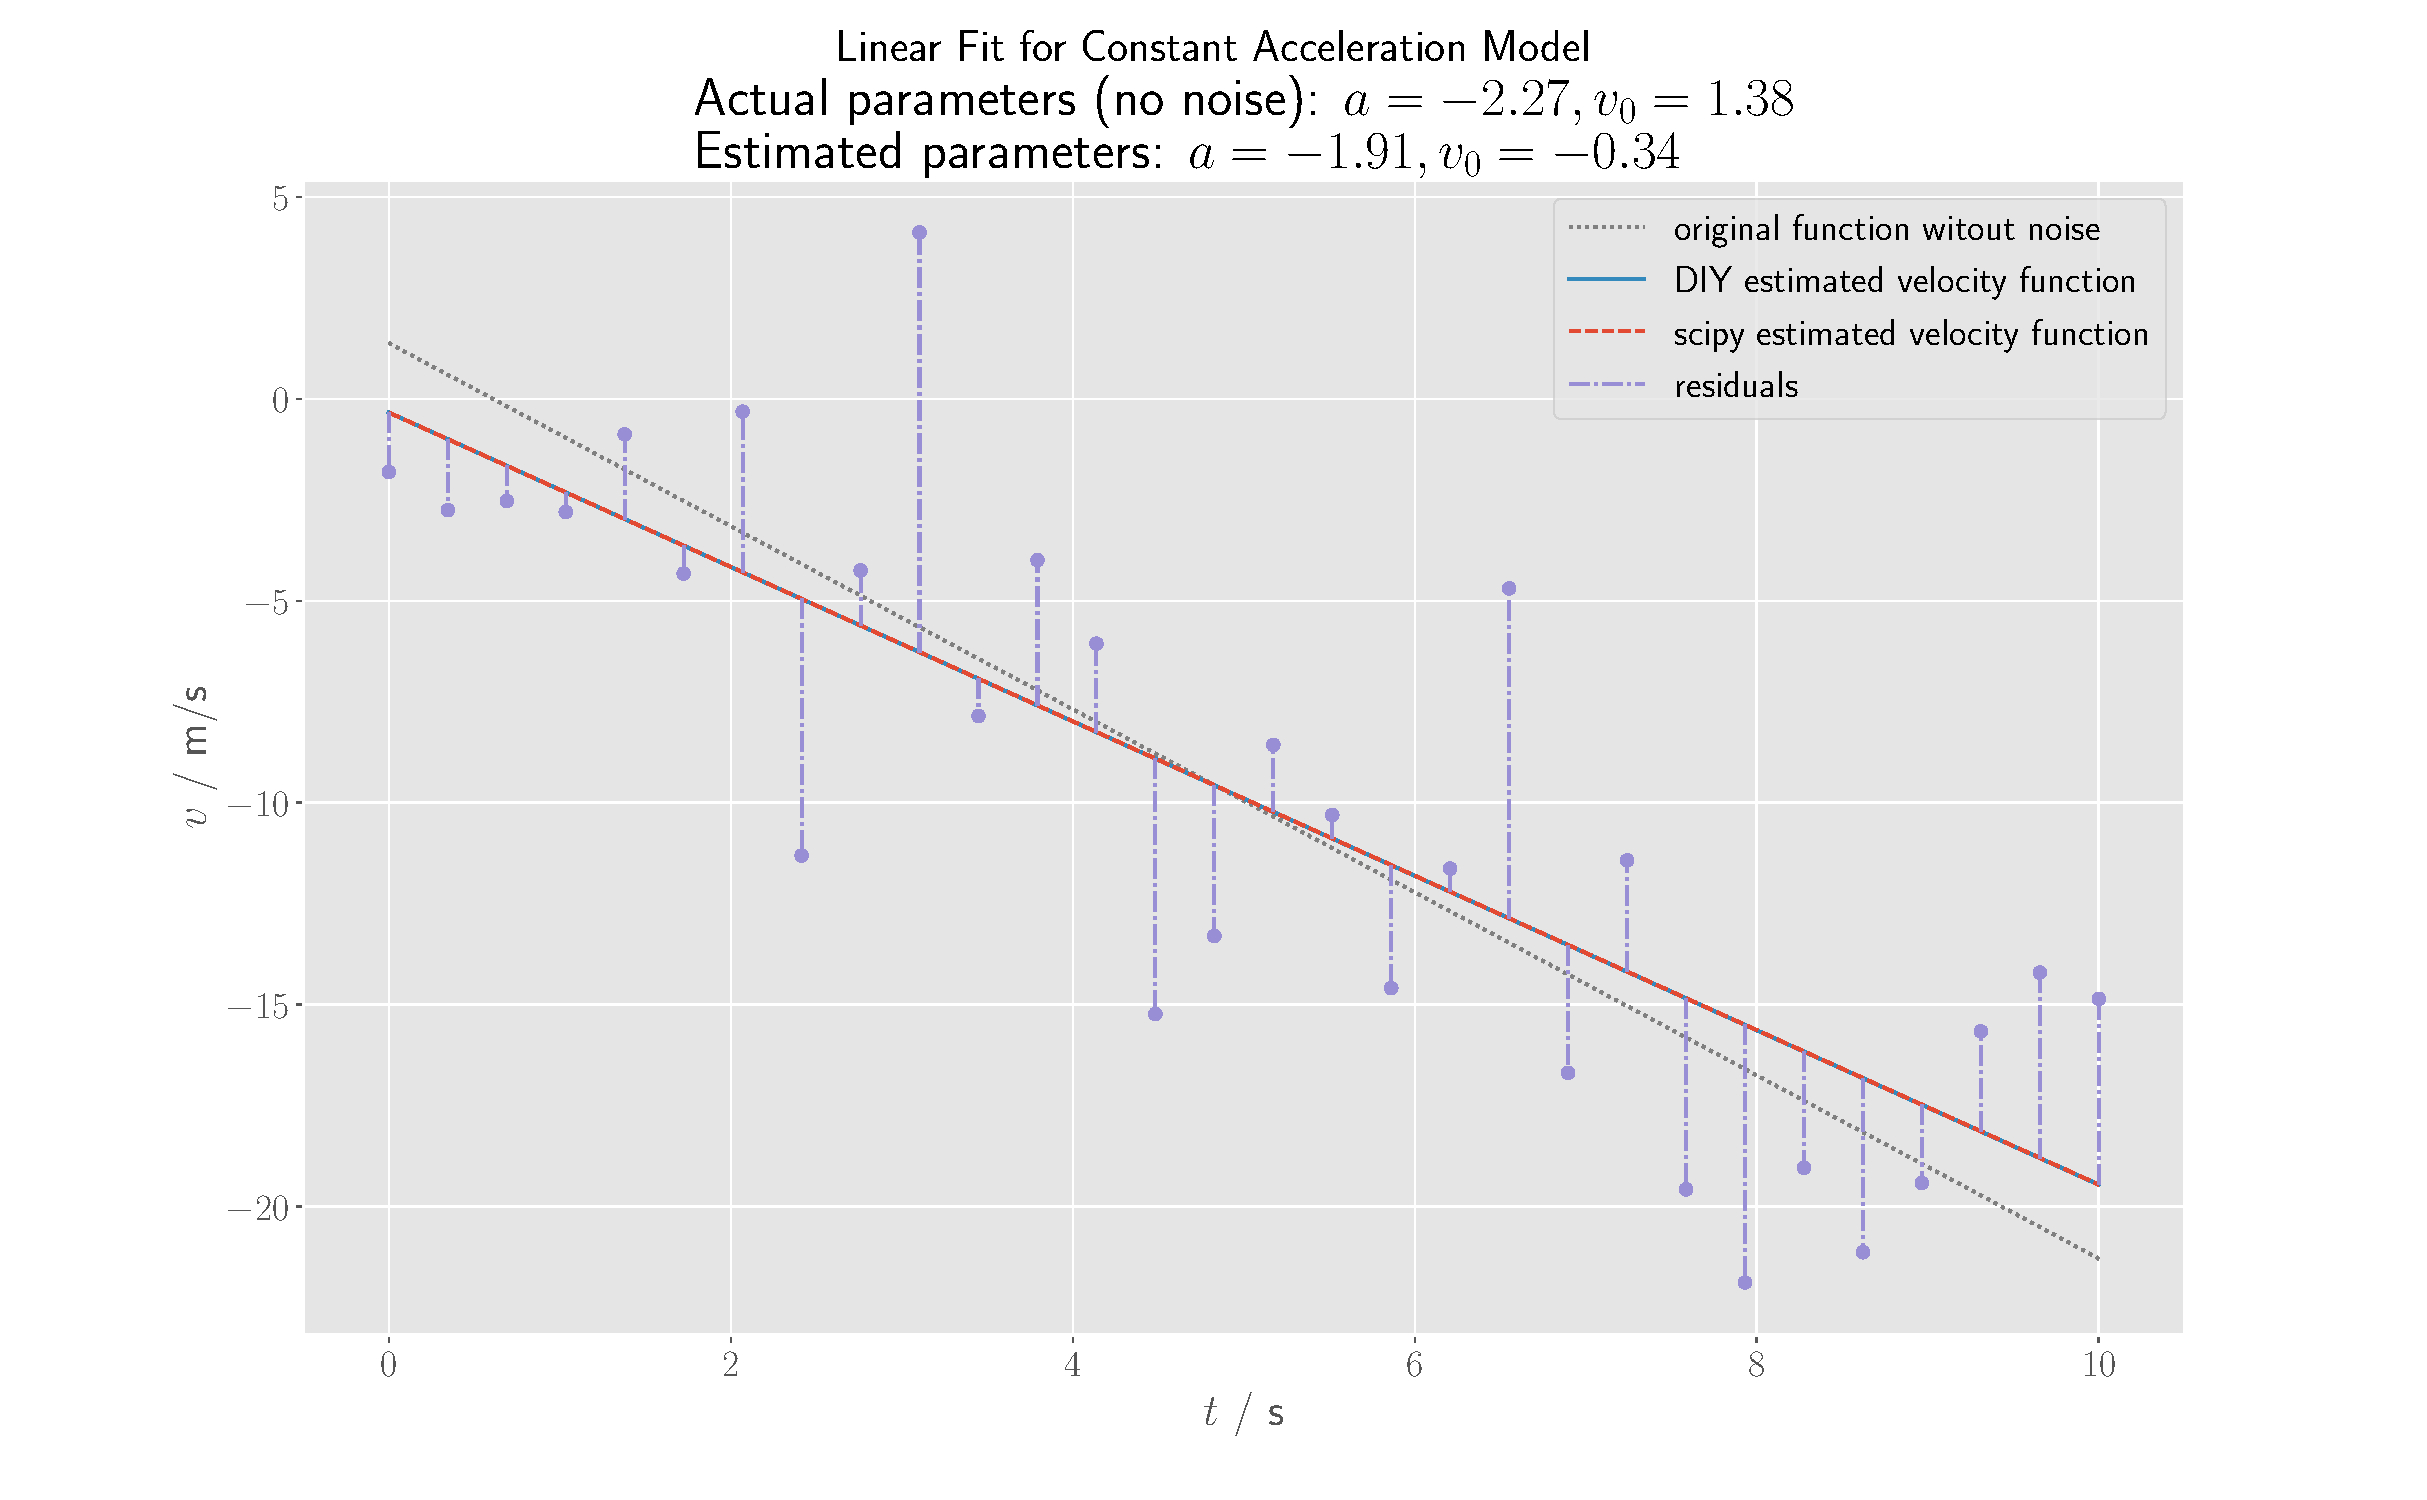
\includegraphics[width=0.764\textwidth]{graphics/linear_fit_1.pdf}
  \caption{Result of fitting the noisy velocity data with a linear model function.}\label{fig:linear}
\end{figure}


\subsection{Decelerating Car}
The speed of a decelerating car will be modeled by the following equation. \cite{stack_car}

\[
  v(t) = A \cdot e^{-b\cdot t} + c
\]

Consequently, the integral of this will result in the distance traveled
\[
  d(t) = \frac{v_{0}}{k}\cdot\left(1 - e^{-k\cdot t}\right) + d_{0}
\]

An exponential fit can actually be found using a linear model function as a helper, given some extra steps.
We take the natural logarithm of $d(t)$ and substitute the parameters of the then linear equation: \cite{brandt_data}
\[
  \underbrace{\ln{d(t)}}_{y(t)} = \underbrace{\ln{a}}_{x_{1}} + \underbrace{b}_{x_{2}} \cdot t
\]

After supplying this to the linear model, we can perform the inverse operations (exponentiation) to get the wanted parameters. In this case, \inlinecodee{scipy.optimize.curve\_fit} was used, so that one can simply define the function to be optimized, making the substituion unnecessary. Figure \ref{fig:expo} shows the result. This assumes that the velocity data can actually be negative.\\

\begin{figure}[h]
  \centering
  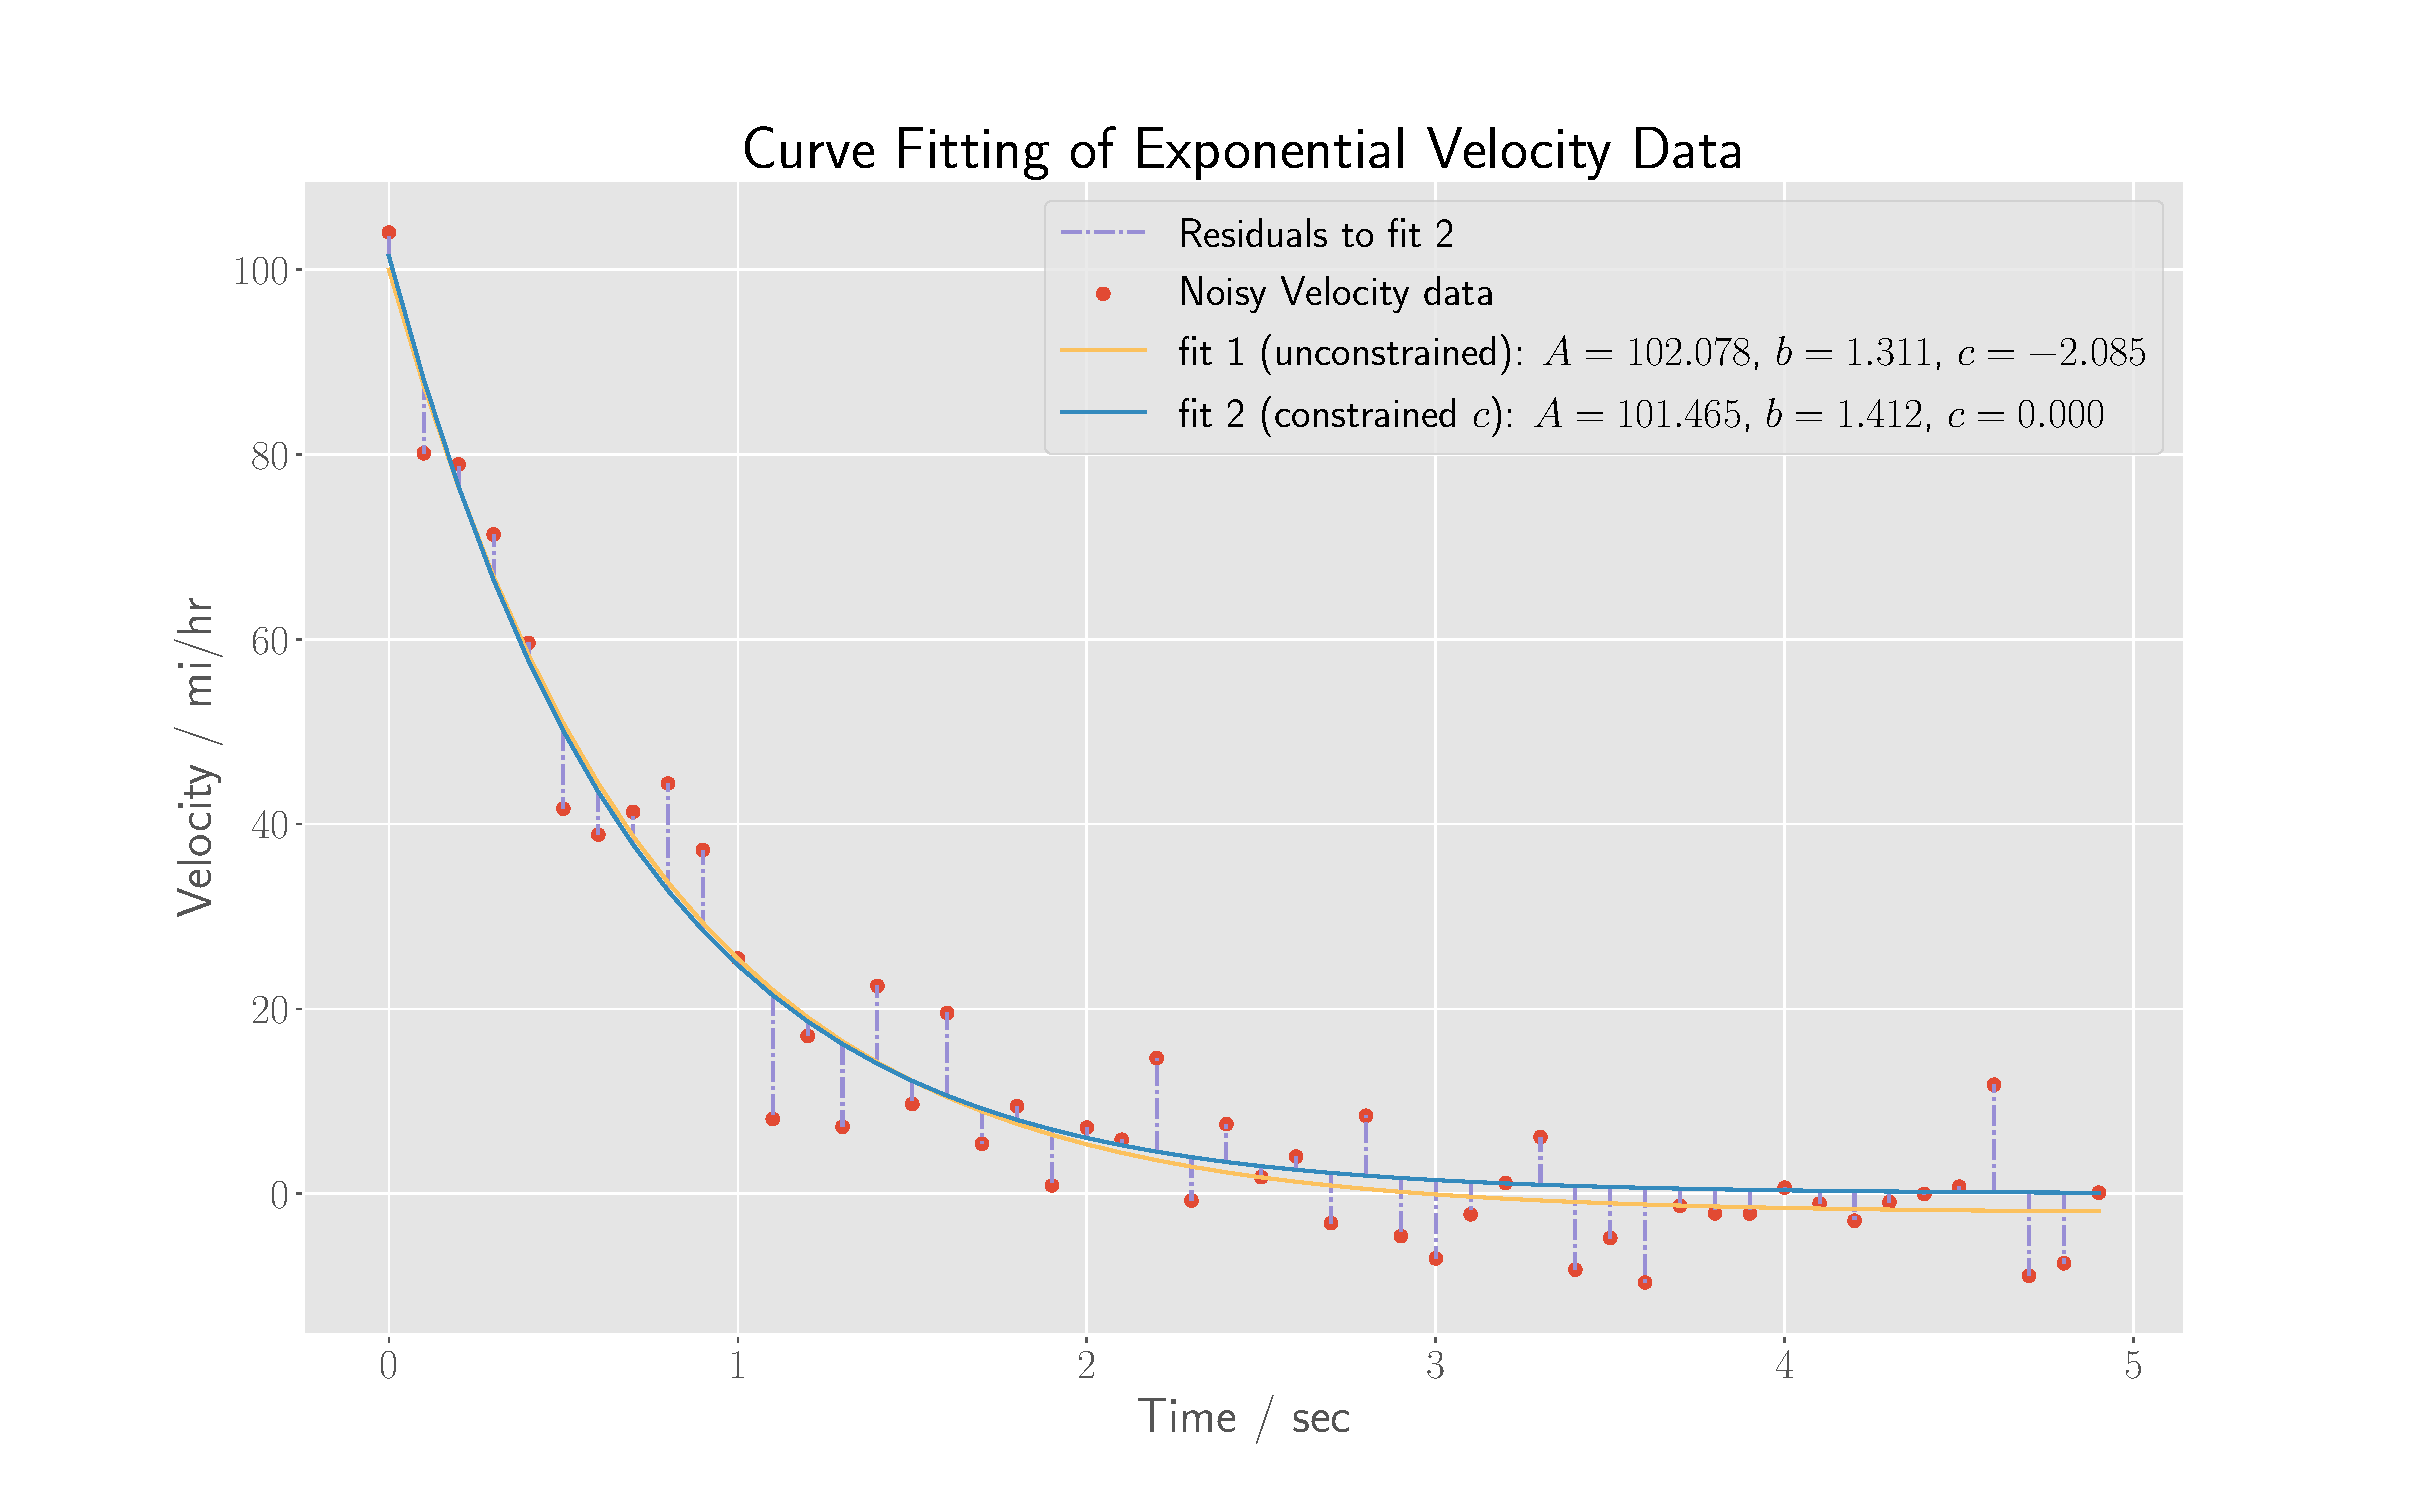
\includegraphics[width=0.764\textwidth]{graphics/exp_fit.pdf}
  \caption{Result of fitting the noisy exponential velocity data.}\label{fig:expo}
\end{figure}


When fitting exponential models, it might be necessary to constrain the additional y-offset parameter to zero if we know that our data actually decays to zero. However, it could also be that the time constant of a model with non zero y-offset more closely matches our system. This has to be adjusted based on the specific application.

\subsection{Periodic Temperature Variation}
The curve fitting of this kind of problem is again very straight-forward using \inlinecodee{scipy.optimize.curve\_fit}.
The adjustable parameters for the sinusoidal function are amplitude, frequency, phase, and offset. The result can be seen in figure \ref{fig:sin}.\\

\begin{figure}[h]
  \centering
  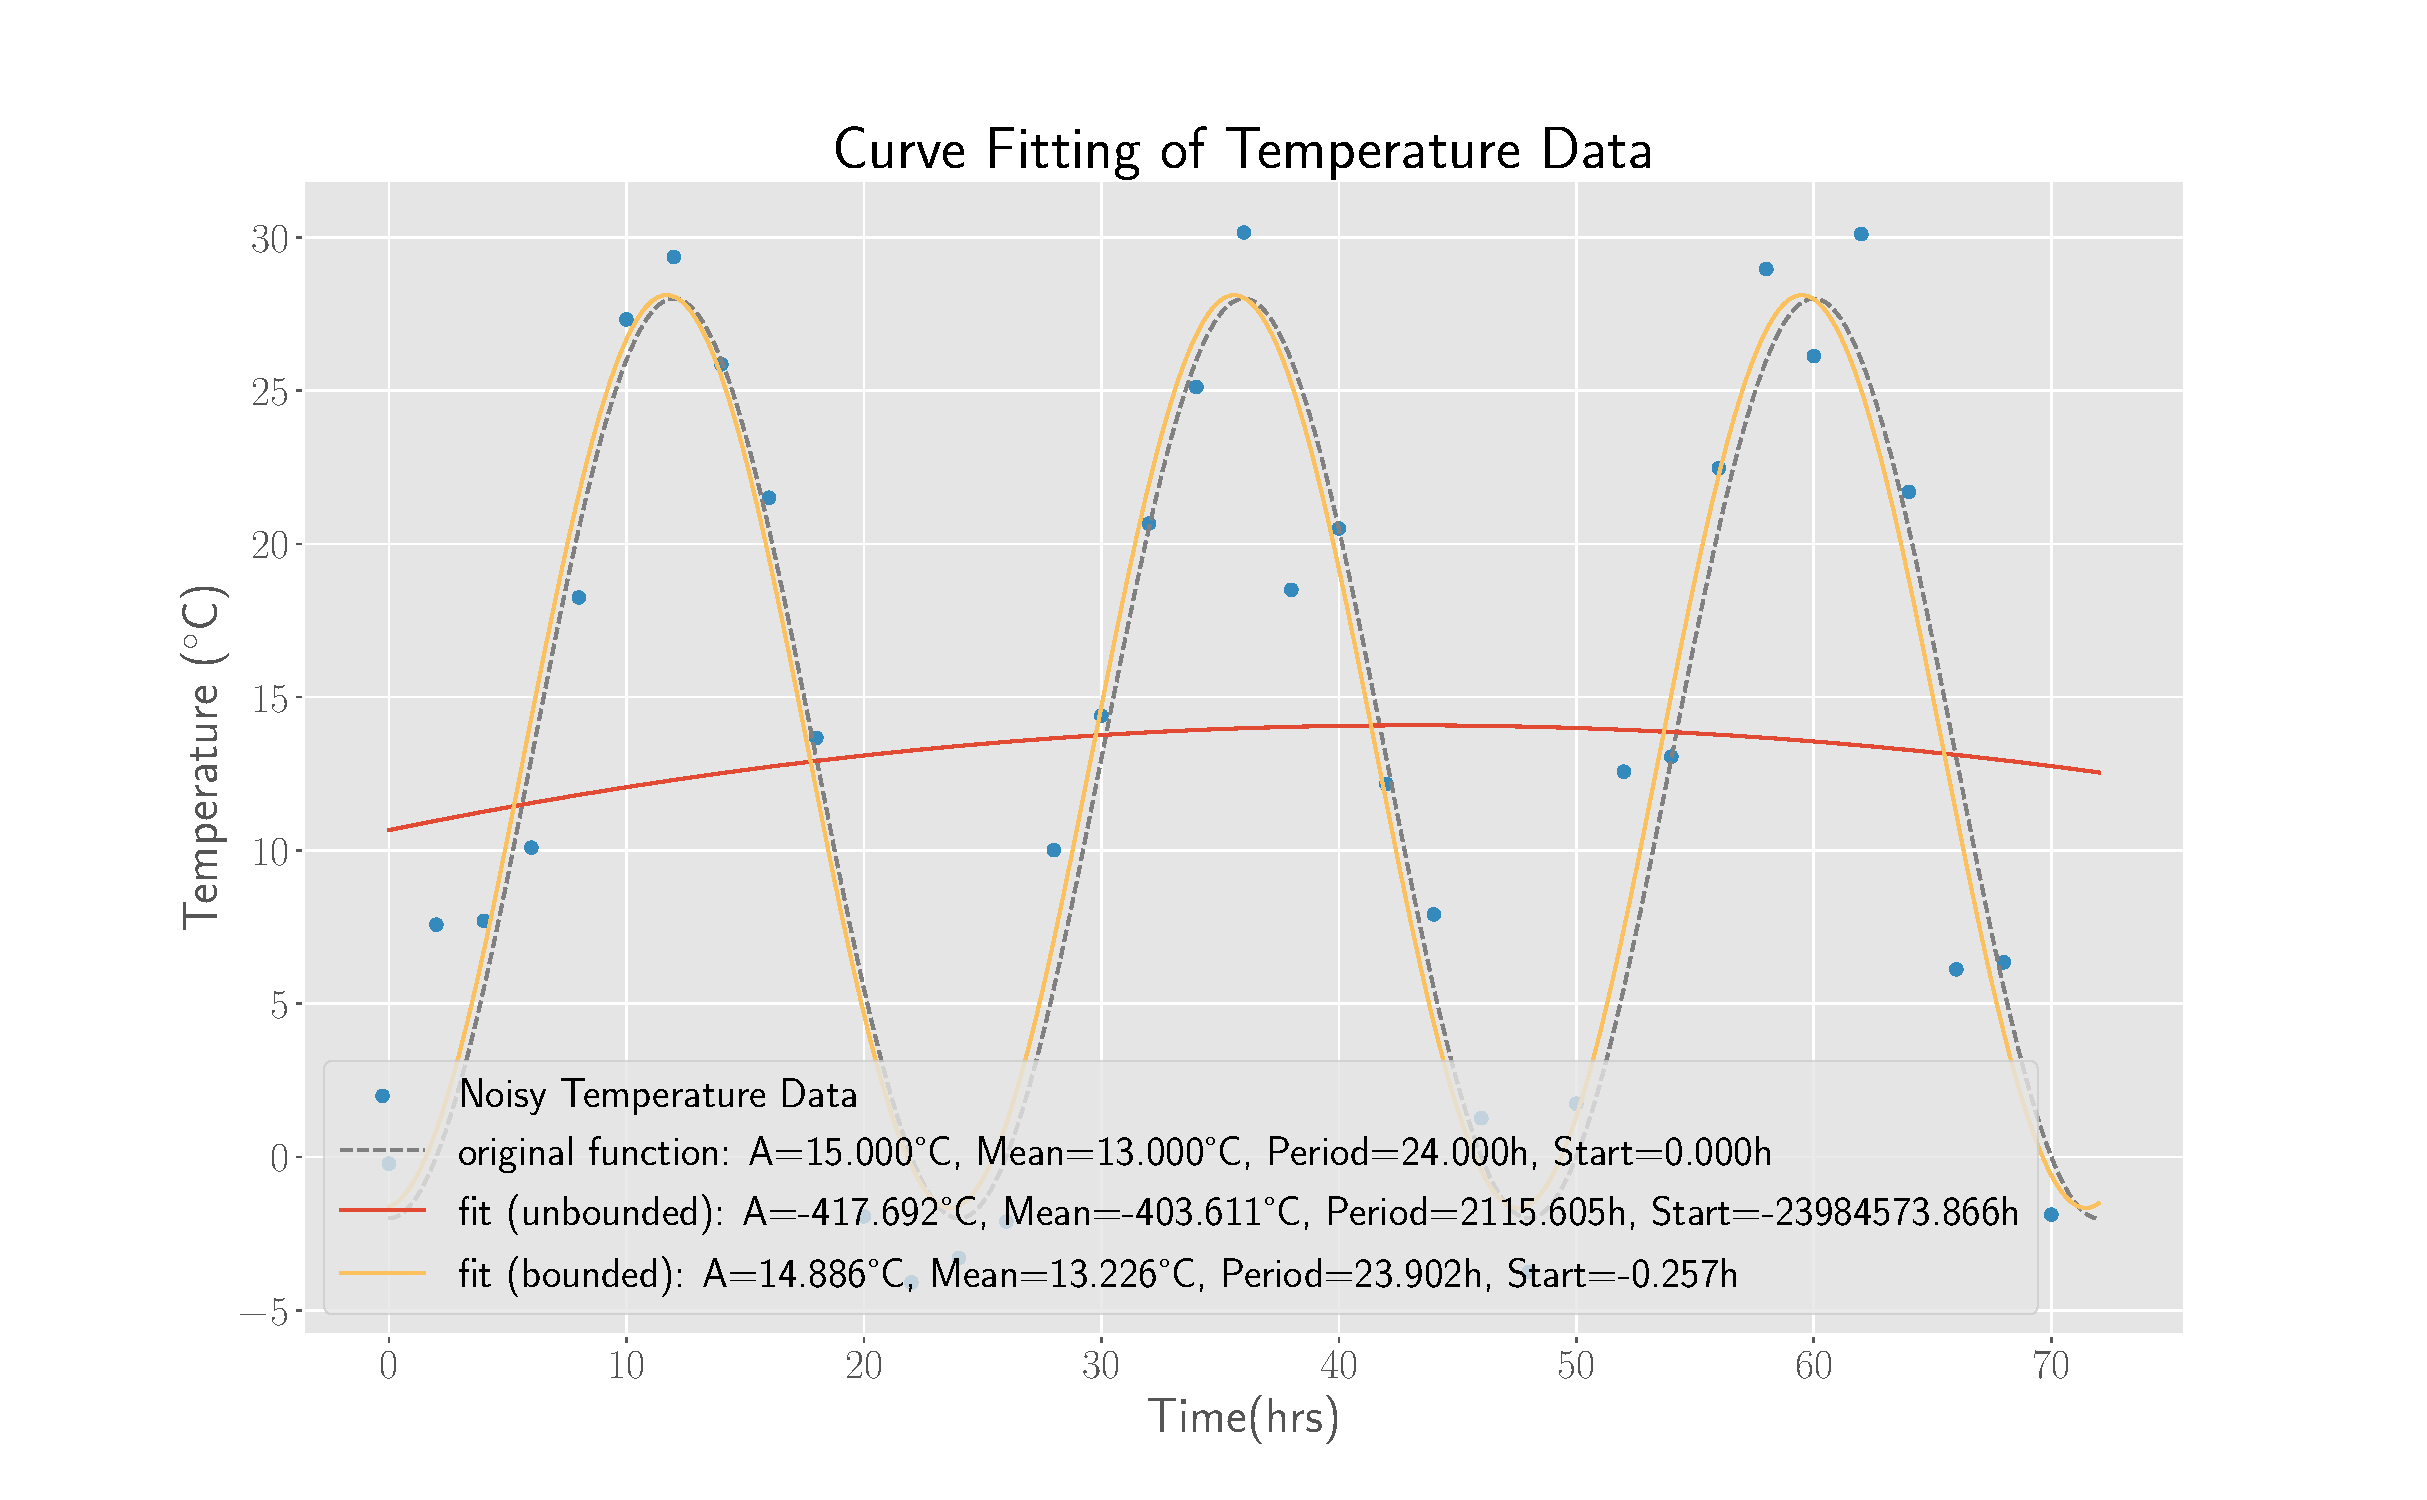
\includegraphics[width=0.764\textwidth]{graphics/sin_fit.pdf}
  \caption{Result of fitting the noisy periodic temperature data.}\label{fig:sin}
\end{figure}

Figure \ref{fig:sin} also shows a problem with using the \inlinecodee{curve\_fit} function without first providing bounds on the decision variables. In this case, the period had to be relatively tightly bound to an interval of $[18\,\si{\hour},24\,\si{\hour}]$ to make the optimization produce a reasonable fit.


\subsection{Randomly Distributed Variable}
As required, a random discrete distribution of numbers from 0 to 10 was generated, where all values except $6$, $7$ and $8$ are uniformly distributed. $6$ and $8$ appear with double the probability of the other values ($12.5\,\si{\percent}$) and $7$ with $4$ times the probability ($25\,\si{\percent}$). This was done by allocating all the numbers with their specific proportion and then picking a random entry from this allocation (see appendix \ref{app:gauss}). %The resulting density histogram for $10000$ random values can be seen in figure \ref{fig:gauss1}.

\begin{figure}[h]
  \centering
  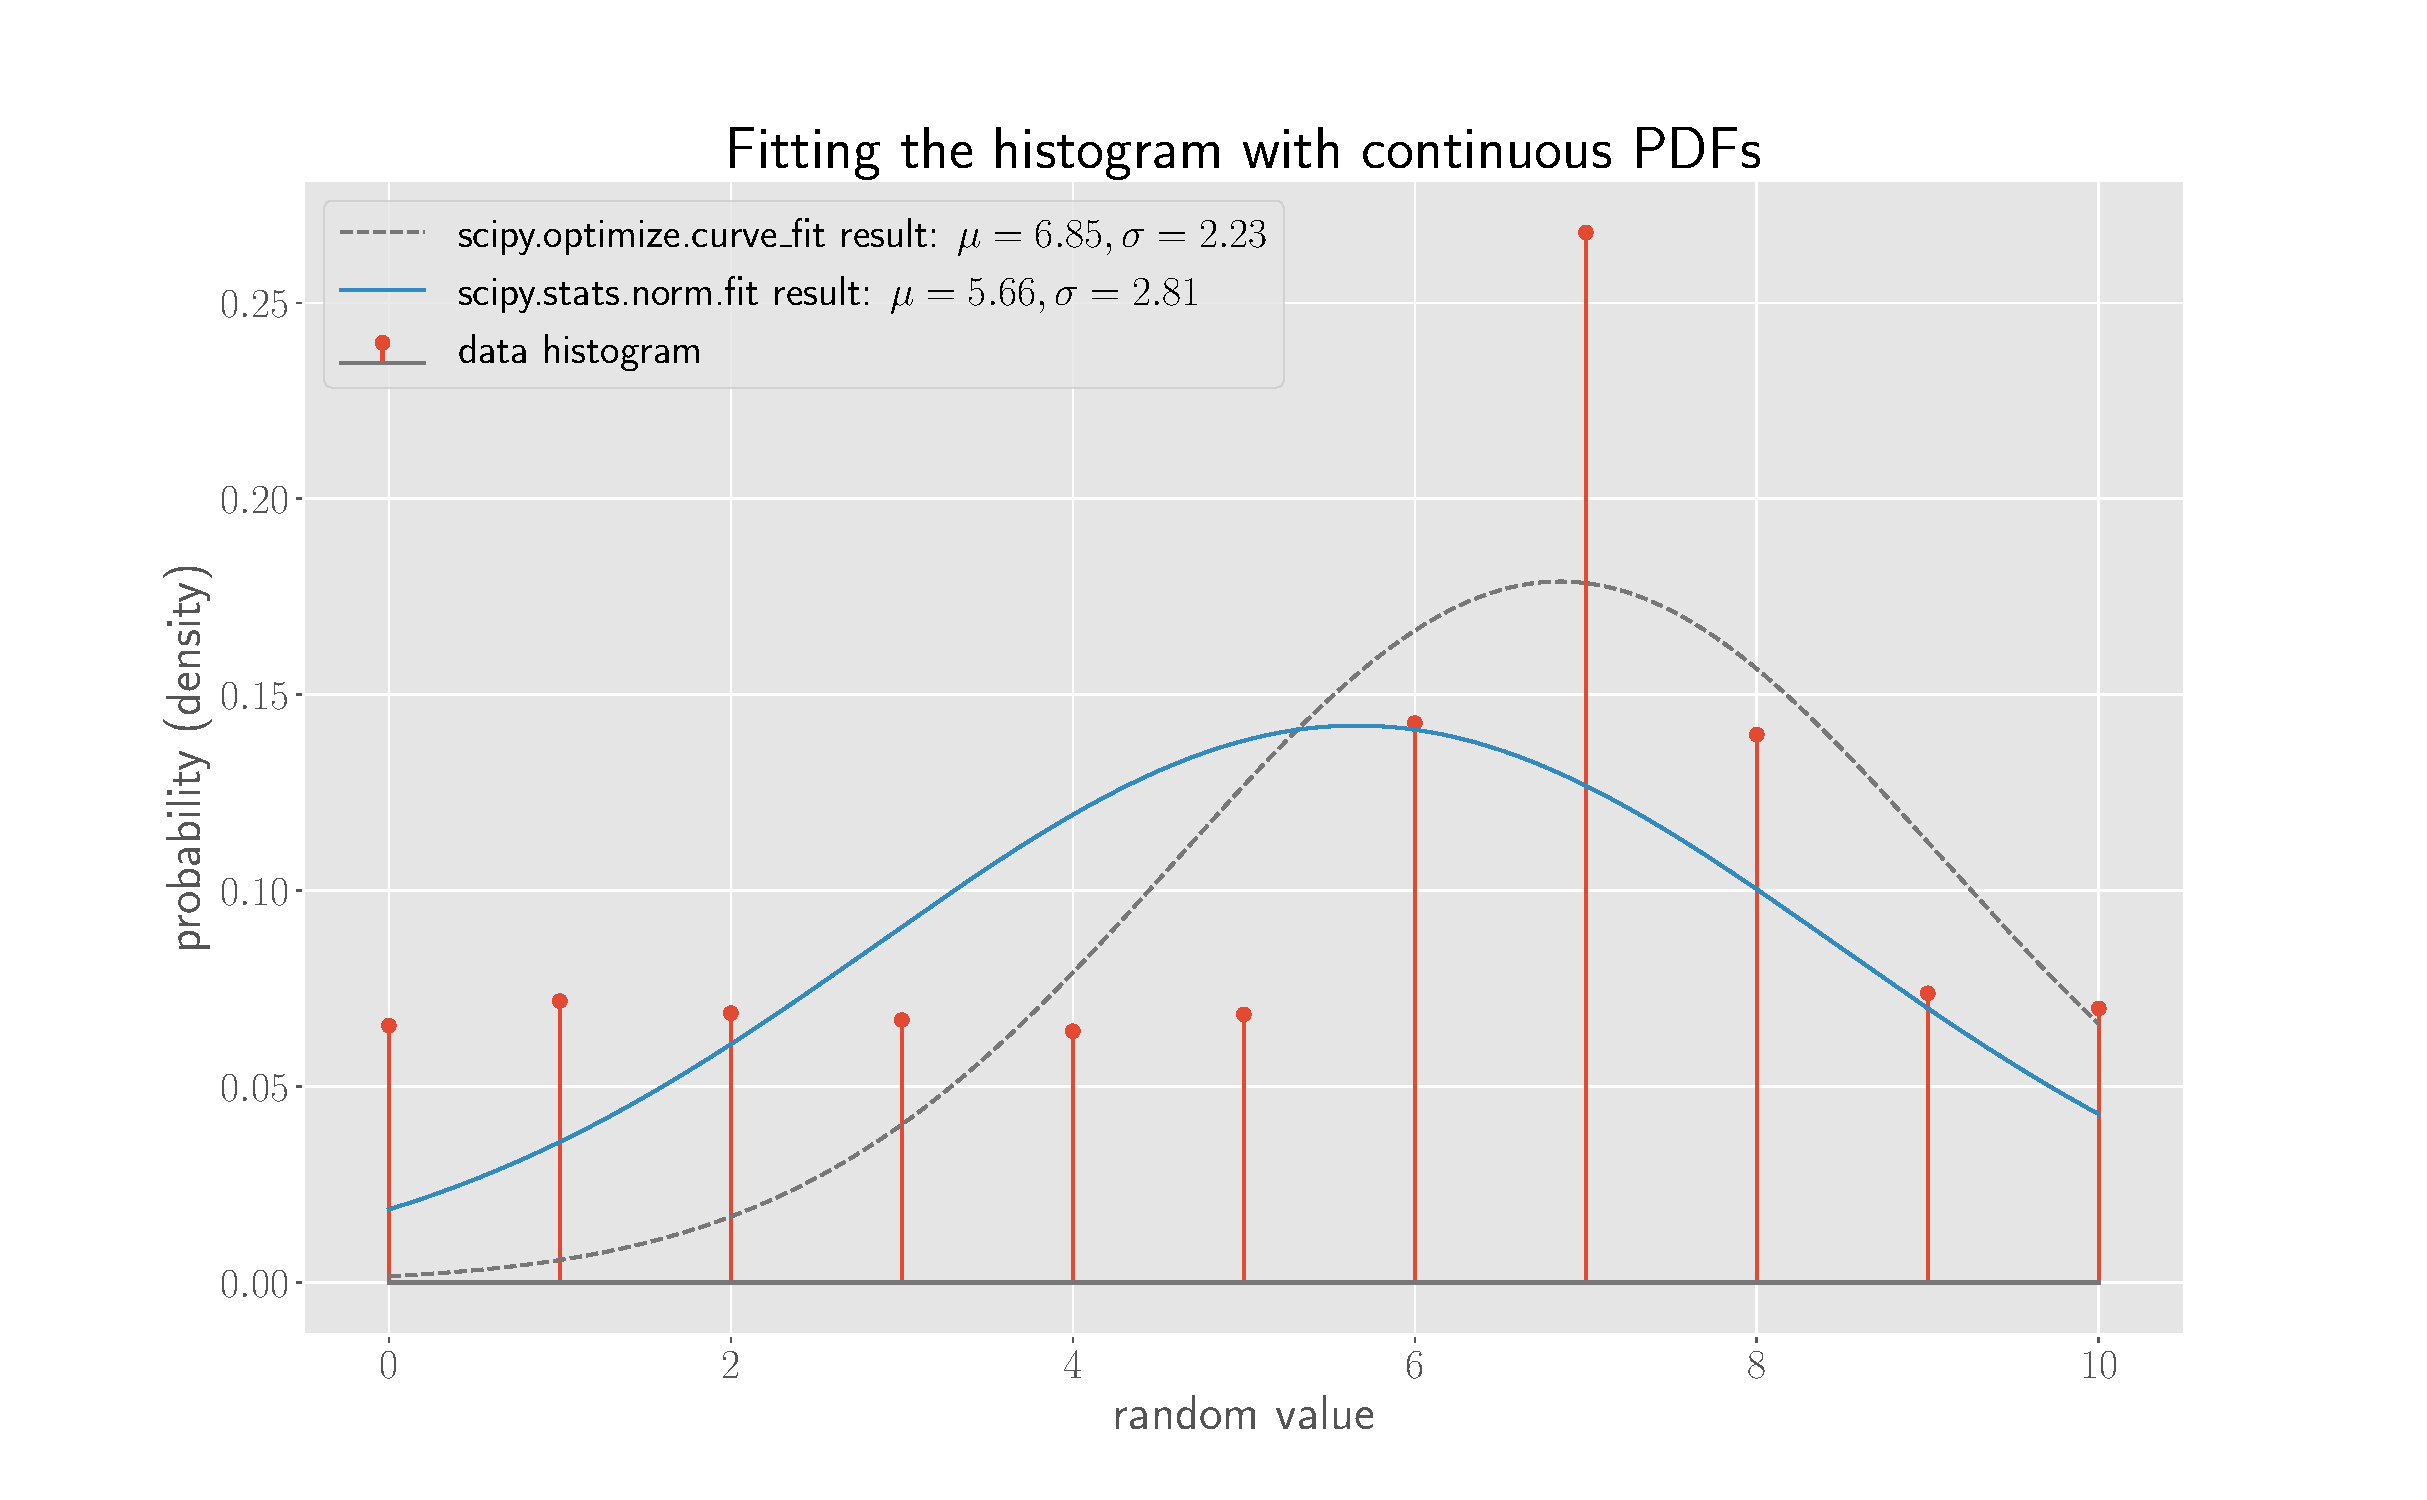
\includegraphics[width=0.764\textwidth]{graphics/gauss_cont.pdf}
  \caption{Fitting the discrete histogram data points with continuous PDF functions. Once with \inlinecodee{optimize.curve\_fit} (as before) and once with \inlinecodee{stats.norm.fit}.}\label{fig:gauss1}
\end{figure}


The problem with this is that trying to fit a continuous gaussian curve to the histogram data (by mean squared error) does not make much sense, mathematically. It is known that our random variable is discrete and can only take on values in the range of 0 to 10. The simple gaussian distribution fit will create a significant area outside of this interval, i.e. the area in the interval is not equal (or close) to 1. Secondly, the values (bins) of $9$ and $10$ close to the ``mean value'' $7$ will have a probability that is much greater than those of the first bins ($0, 1, 2, ...$), even though they should be close to equal which can be seen by a quick estimation of the area under the function (figure \ref{fig:gauss1}).\\

The solution is to use a method of dedicated ``probability distribution fitting'' such as the \textit{Maximum likelihood estimation} and constrain the problem to a discrete distribution. Scipy implements this in \inlinecodee{scipy.stats.fit}, where a certain distribution type can be passed. \cite{scipy_doc_dist_fit} For discrete distributions, it is a little bit more complicated, as a proper distribution function is not as easily found. For this kind of constructed scenario, the values follow a \textit{multinominal distribution}, a discrete distribution where each value (or group) is associated with a distinct probability. The probability mass function of this is given by (see \cite{scipy_doc_multinominal})
\[
  f(x) = \frac{n!}{x_1! \cdots x_k!} p_1^{x_1} \cdots p_k^{x_k},
\]

One could define a cost function that determines how far the specific distribution (PMF) deviates from the data. Then use that to perform a minimization optimization. However, this is not really useful in this case, as one might as well just use the values from the histogram.

% All of this is to say that there is not really a point in fitting this kind of discrete distribution.% \footnote{A good video tutorial on this matter can be found at \url{https://www.youtube.com/watch?v=TwbJCt36_DU}.}

\section{Conclusions}
A few different curve fitting problems have been studied. \inlinecodee{scipy.optimize.curve\_fit} provides a useful tool for this kind of task since it is very flexible regarding custom function definitions. Nevertheless, one has to be clear about the origin of their data and their intent when fitting to be able to make realistic predictions.


\printbibheading

%\printbibliography
\begin{refsection}[sources.bib]
\nocite{*}
\printbibliography[heading=subbibliography,title={Literature}]
\end{refsection}

\begin{refsection}[software.bib]
\nocite{*}
\printbibliography[heading=subbibliography,title={Software Used}]
\end{refsection}

\pagebreak
\appendix
\section{Python Code}\label{app:script}

\subsection{Linear Fit}\label{app:linear}
\inputminted{python}{./code/linear_fit.py}

\pagebreak
\subsection{Exponential Fit}\label{app:exponential}
\inputminted{python}{./code/exponential_fit.py}

\pagebreak
\subsection{Sinusoidal Fit}\label{app:sinusoidal}
\inputminted{python}{./code/sin_fit.py}

\pagebreak
\subsection{Probability Distribution Fit}\label{app:gauss}
\inputminted{python}{./code/gaussian_fit.py}

\end{document}
